\section{Properties of the Wigner distribution}
\label{app:wigner}

Here we present important properties of the Wigner distribution that are used throughout the paper.

\begin{proposition}\label{thm:wstate}
    The Wigner distribution of a state $\rho$ is
    \begin{enumerate}
        \item\label{en:w1} Real valued: $\W{\rho} \in \mathbb{R}^{d^2}$;
        \item\label{en:w2} Normalised: $\sum_{\bmz \in \pd} \W[\bmz]{\rho}=1$;
        \item\label{en:w3} Bounded: $\abs{\W[\bmx]{\rho}} \leq \frac{1}{d}$.
        \item\label{en:w4} Additive under mixing:
        
        $\W[\bmx]{\sum_i p_i \rho_i} = \sum\limits_i p_i \W[\bmx]{\rho_i}$;
        \item\label{en:w5} Multiplicative under tensor products: 
        
        $\W[\bmx_A \oplus \bmx_B]{\rho_A \otimes \rho_B} = \W[\bmx_A]{\rho_A}\W[\bmx_B]{\rho_B}$.
	\end{enumerate}
\end{proposition}
A distribution satisfying the first three properties does not necessarily correspond to a positive semi-definite state.

\begin{proposition}
    \label{thm:wchannel}
    The Wigner distribution of a $\cptp$ operation $\E: \cal{B}(\hd[d_A]) \mapsto \cal{B}(\hd[d_B])$ is:
    \begin{enumerate}
        \item\label{en:wo1} Real-valued: $\W[\bmy|\bmx]{\E} \in \mathbb{R}$;
        \item\label{en:wo2} Normalised: $\sum_{\bmz \in \pd[d_B]} \W[\bmz|\bmx]{\E} = 1$ for any $\bmx \in \pd[d_A]$;
        \item\label{en:wo3} Bounded: $\abs{\W[\bmy|\bmx]{\E}} \leq \frac{d_A}{d_B}$;
	    \item\label{en:wo4} \nick{Transitive}: $\W[\bmy]{\E(\rho)} = \sum_{\bmz \in \pd[d_A]} \W[\bmy|\bmz]{\E} \W[\bmz]{\rho}$ for any $\bmy \in \pd[d_B]$.
    \end{enumerate}
\end{proposition}
If $d_A = d_B$, and in particular if operation $\E$ maps a Hilbert space onto itself, then the stochasticity condition $\abs{\W[\bmy|\bmx]{\E}} \leq 1$ is satisfied.

%%%

\section{Properties of majorization}
\label{app:major}

\subsection{Equivalent conditions for majorization}

Any $\bmd$-majorization problem can be rephrased as a majorization problem in a higher dimensional space due to the embedding map.
\begin{definition}
    The embedding map $\Gamma_{\bmd}:\mathbb{R}^n \mapsto \mathbb{R}^D, D = \sum\limits_{i=1}^n d_i$ is the function
    \begin{equation}
        \Gamma_{\bmd}(\bmz) = \bigoplus_{i=1}^n z_i\  \frac{1}{d_i}\bm{1},
    \end{equation}
    where $\bm{1}/d_i$ is the $d_i$-dimensional uniform distribution.
    The left inverse $\Gamma_{\bmd}^{-1}: \mathbb{R}^D \mapsto \mathbb{R}^n$ is defined to sum up the elements in each block of $\Gamma_{\bmd}(\bmz)$, so that
    \begin{equation}
        \Gamma_{\bmd}^{-1}(\oplus_{i=1}^n z_i \bm{1}/d_i) = \bmz.
    \end{equation}
    This is not a right inverse, because $\Gamma_{\bmd}$ is not surjective.
\end{definition}
The direct sum simply amounts to listing the uniform distributions one after the other.
The embedding map maps the Gibbs distribution to the uniform distribution, $\Gamma_{\bmd}(\bmd) = \bm{1}/D$.
Then, a non-increasing ordering $\Gamma_{\bmd}(\bmz)^\downarrow$ in the new space, corresponds to the so-called ``$\beta$-ordering'' of the original vector denoted by the permutation $\pi$ mapping $(z_i/d_i) \mapsto (z_i/d_i)^\downarrow$ for all $i=1,\dots,n$.
Intuitively, $\beta$-ordering tends to simply non-increasing ordering as $\beta$ tends to 0.
This ordering naturally leads to a generalised notion of the Lorenz curve. 

\begin{theorem}
Given $\bmx, \bmy, \bmd \in \mathbb{R}^n$, such that the components of $\bmd$ are positive, the following statements are equivalent:
 \begin{enumerate}%[\rm{(TM1)}]
	\item $\bmx \prec_{\bmd} \bmy$;
	\item $\Gamma_{\bmd}({\bmx}) \prec \Gamma_{\bmd}({\bmy})$;
	\item\label{en:tm3} $\sum\limits_{i=1}^n \abs{x_i - t d_i} \leq \sum\limits_{i=1}^n \abs{y_i - t d_i}$ for all $t \in \mathbb{R}$;
	\item $\sum\limits_{i=1}^n (x_i - t d_i)^+ \leq \sum\limits_{i=1}^n (y_i - t d_i)^+$ for all $t \in \mathbb{R}$ and $\sum\limits_{i=1}^n x_i = \sum\limits_{i=1}^n y_i$;
	\item $\forall k, L_{\bmx|\bmd}(k) \leq L_{\bmy|\bmd}(k)$ and $L_{\bmx|\bmd}(k=n) = L_{\bmy|\bmd}(k=n)$.
 \end{enumerate}
\end{theorem}
\begin{proof}
    \begin{enumerate}
        \item[1$\leftrightarrow2$]
        Suppose now there exists a stochastic $S$ such that $\bmx = S\bmy$ with $\bmd = S\bmd$ and let $B = \Gamma_{\bmd} \circ S \circ \Gamma_{\bmd}^{-1}$.
        $B$ is a $D$-dimensional bistochastic matrix, since composition of stochastic matrices is stochastic and $(\Gamma_{\bmd} \circ S \circ \Gamma_{\bmd}^{-1}) (\frac{1}{D}\bm{1}) = (\Gamma_{\bmd} \circ S) (\bm{d}) = \Gamma_{\bmd}(\bm{d}) = \frac{1}{D}\bm{1}$. Then, $B$ maps $\Gamma_{\bmd}({\bmy})$ to $\Gamma_{\bmd}({\bmx})$.
        Conversely, given $B$, let $S = \Gamma_{\bmd}^{-1} \circ B \circ \Gamma_{\bmd}$.
        Similarly, $S$ is the stochastic matrix that preserves $\bmd$ and maps $\bmy$ to $\bmx$.
        \item[$2\leftrightarrow3$]\hspace{-5pt}, $2\leftrightarrow4$, $2\leftrightarrow5$ These three statement are equivalent to \nick{blah} respectively for the embedded vectors $\Gamma_{\bmd}({\bmx}), \Gamma_{\bmd}({\bmy})$.
        This is clear by rewriting
        \begin{align}
            \sum\limits_{i=1}^n \abs{x_i - t d_i} &= \sum\limits_{i=1}^n d_i \abs{\frac{x_i}{d_i} - t} = \sum\limits_{i=1}^D \abs{\Gamma_{\bmd}(\bmx)_i - t}, \\
            \sum\limits_{i=1}^n (x_i - t d_i)^+ &= \sum\limits_{i=1}^D (\Gamma_{\bmd}(\bmx)_i - t)^+, \\
            L_{\bmx|\bmd}(k) &= L_{\Gamma_{\bmd}(\bmx)}(k'), \\
            \text{with}\ k&=1,\dots,n\ \text{and}\ k'=1,\dots,D \nonumber
        \end{align} 
        and similarly for the right hand side.
    \end{enumerate}
\end{proof}

The Lorenz curve can be explicitly expressed as
    \begin{equation}
		\lc{\rho}{\sigma}(x) = (\bmu^\downarrow)_i x + \lc{\rho}{\sigma}(i) - (\bmu^\downarrow)_i x_i,\ x \in (x_{i-1}, x_i],
	\end{equation}
	for all $i=1,\dots,d$ with $x_0 \coloneqq 0$.

\subsection{Mana properties}
Mana monotonicity in any $\sigma$--fragment can be directly seen due to statement~\ref{en:tm3} in~\cref{thm:dmajor} for $t=0$.
Furthermore, mana is additive due to the multiplicative property~\ref{en:w4} of~\cref{thm:wstate}.

%%%

\section{Properties of $\sigma$-fragments}
\label{app:frag}

\begin{theorem}\label{thm:frag}
    Let $\R = (\O, \F)$ be a magic theory. 
    The following statements hold:
    \begin{enumerate}
        \item No $\sigma$-fragment is empty.
        \item If a free operation leaves two states invariant, then it also leaves their mixtures invariant, 
        \begin{equation}
            \O_{\sigma} \cap \O_{\sigma'} \subseteq \O_{p\sigma + (1-p)\sigma'}\ \text{for all}\ p \in [0,1].
        \end{equation}
        \item Let $\E$ be a $\cptp$ operation with Wigner distribution $\W{\E}$.
        For $\R = \Rmax$ $\E \in \O_\sigma$ iff $\W{\E} \in \stochw$.
    \end{enumerate}
\end{theorem}
\begin{proof}$ $\\

    \begin{enumerate}
    \item The identity channel $1_{\rm{C}}: \D \mapsto \D$ belongs to every $\sigma$-fragment, as $1_{\rm{C}} \in \O$ and $1_{\rm{C}}\sigma = \sigma$ for all $\sigma \in \F$.
    
    \item Let $\E \in \O_{\sigma} \cap \O_{\sigma'}$.
    Then $\E \in \cptp$ and corresponds to stochastic Wigner distribution $\W{\E}$ such that $\W{\E} \W{\sigma} = \W{\sigma}$ and $\W{\E} \W{\sigma'} = \W{\sigma'}$.
    Then, $\W{\E} \W{p\sigma + (1-p)\sigma'} = \W{p\sigma + (1-p)\sigma'}$ for any $p \in [0,1]$ due to the additive property~\ref{en:w4} of the Wigner distribution, implying that state $p\sigma + (1-p)\sigma'$ is also left invariant by $\E$.
    
    \item Let $\O_\sigma' \coloneqq \{ \E \in \cptp: \W{\E} \in \stochw \}$ be the described set of operations.
    
    Suppose $\E$ is in $\O_\sigma$, then $\E \in \cptp$ and $\W{\E} \in \stochw$ due to property~\ref{en:wo4} of~\cref{thm:wchannel}, hence $\O_\sigma \subseteq \O_\sigma'$.
    
    Conversely, suppose $\E \in \cptp$ with $\W{\E} \in \stochw$. 
    Then, $\W[\bmy|\bmx]{\E} \geq 0$ for all $\bmx, \bmy$, hence $\E \in \O$.
    Furthermore, $\W{\E} \W{\sigma} = \W{\sigma}$ implies $\E(\sigma) = \sigma$ using~\cref{eq:woperation} defined for any $\cptp$ operation $\E$.
    Hence, $\O_\sigma' \subseteq \O_\sigma$.
    \end{enumerate}
\end{proof}

Any free state $\sigma \in \cal{B}(\hd)$ corresponds to a $d^2$-dimensional probability distribution $\W{\sigma}$ and any free operation $\E: \cal{B}(\hd) \mapsto \cal{B}(\hd)$ corresponds to a $d^2 \times d^2$ stochastic matrix (or conditional probability distribution) $\W{\E}$.
Note that these mappings are one-to-one due to the orthogonality of the phase-point operators as an operator basis.

\emph{Remark 1.} Note that free states $\F$ are mapped onto a \emph{strict subset} of the set of probability distributions.
As a counterexample, the sharp $d^2$-dimensional probability distribution $(1, 0, \dots, 0)$ does not correspond to any qudit Wigner distribution because of the boundedness condition~\ref{en:w3} in~\cref{thm:wstate}.

\emph{Remark 2.} Similarly, not all stochastic matrices correspond to completely positive operations.

As an example, consider the permutation matrix
\begin{equation}
    \Pi_X = \begin{psmallmatrix}
        0 & 1 & 0 & 0 & 0 \\
        0 & 0 & 0 & 0 & 1 \\
        0 & 0 & 0 & 1 & 0 \\
        1 & 0 & 0 & 0 & 0 \\
        0 & 0 & 1 & 0 & 0
    \end{psmallmatrix} \otimes \begin{psmallmatrix}
        0 & 0 & 1 & 0 & 0 \\
        0 & 0 & 0 & 0 & 1 \\
        0 & 0 & 0 & 1 & 0 \\
        1 & 0 & 0 & 0 & 0 \\
        0 & 1 & 0 & 0 & 0    
    \end{psmallmatrix} \in \stochw,\ d=5.
\end{equation}
It preserves the uniform distribution $\W{\frac{1}{5}\id}{}$, but it does not correspond to any $\cpos$ operation, hence any $\E \in \O$ due to~\cref{thm:frag}.

\section{Area monotone}
\label{app:areamono}

Let $L_{>1}$ be the set of points on the Lorenz curve $\lc{\rho}{\sigma}(k)$ that lie above $1$ of state $\rho$ in the $\sigma$--fragment. 
If $\rho$ is a free state, $L_{>1}$ is empty and $\A_\sigma(\rho) = 0$. 
Otherwise, $\A_\sigma(\rho) > 0$ and it can be calculated exactly using the trapezium rule or the shoelace formula. 
Let $k$ be the index of the first point $\left(x_k, \lc{\rho}{\sigma}(k)\right)$ lying above $1$. 
Then $L_\rho(k)$ crosses $1$ at
\begin{equation}
	x_{\rm{int}} = x_k - \frac{x_k - x_{k-1}}{\lc{\rho}{\sigma}(k) - \lc{\rho}{\sigma}(k-1)}\lc{\rho}{\sigma}(k),\vspace{10pt}
\end{equation}
as well as at $\left(x_d, \lc{\rho}{\sigma}(d)\right) = (1,1)$

Now we can define
\begin{equation}
L_{>1}^+ = \{ (x_i, y_i) \}_{0 \leq i \leq n}
\end{equation}
such that it contains the initial point of intersection $(x_0, y_0) \equiv (x_{n+1}, y_{n+1}) \coloneqq (x_{\rm{int}}, 1)$, all points $(x_i, y_i)$, labelled by $i=1,\dots,n-1$ that lie above $y=1$ contained in $L_{>1}$ and finally the second point of intersection $(x_n, y_n) = (1,1)$.
Then, 
\begin{equation}
	\A_\sigma(\rho) = \frac{1}{2} \sum\limits_{i=0}^n (x_{i+1} y_i - x_i y_{i+1}).
\end{equation}

\begin{figure}%
    \centering
    \subfigure[][]{%
    \label{fig:test1}%
    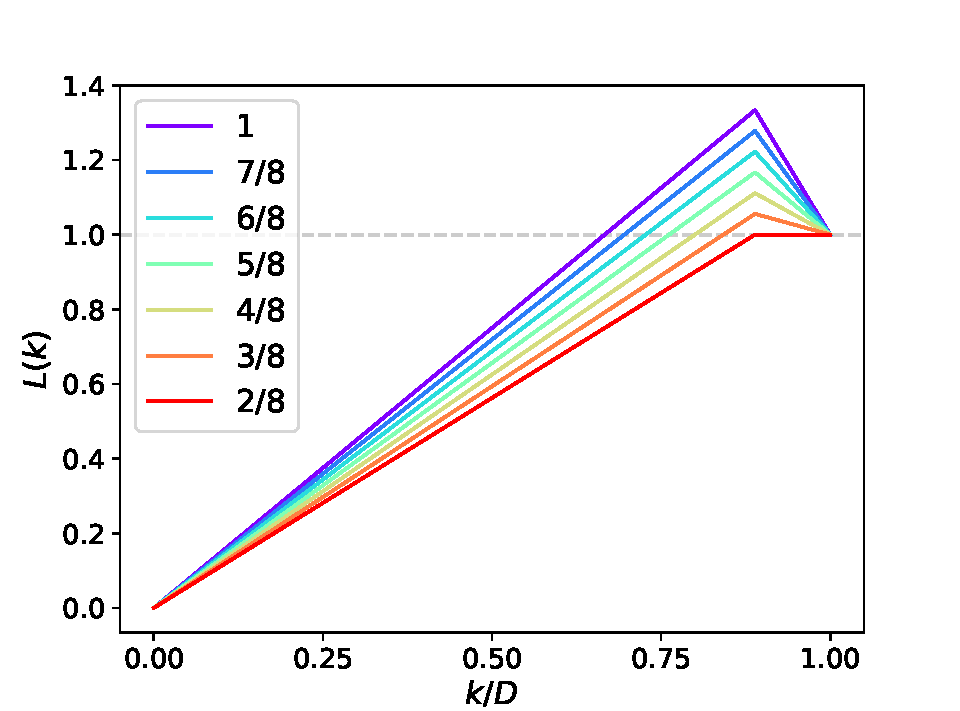
\includegraphics[height=3cm]{figs/negmasking_rho_strange_lc.pdf}
    %\caption{Maximally mixed state $\frac{1}{3}\id$}%
    }\hspace{8pt}%
    \subfigure[][]{%
    \label{fig:test2}%
    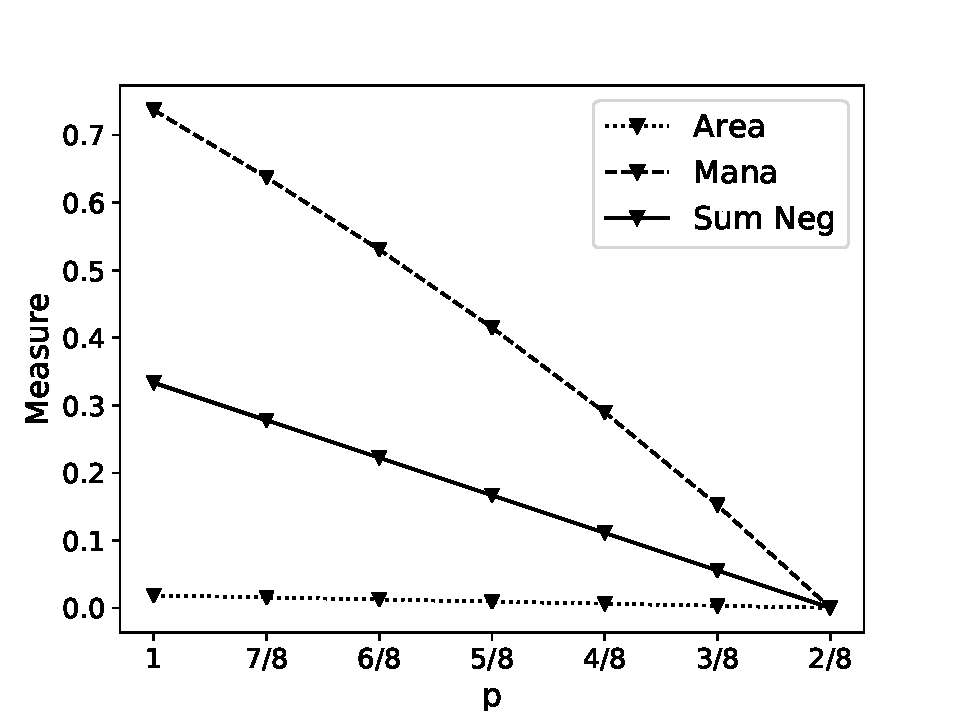
\includegraphics[height=3cm]{figs/negmasking_rho_strange_meas.pdf}
    %\caption{Zero state $\ketbra{0}{0}$}%
    }
    \caption{\subref{fig:test1} Lorenz curve of $p\ketbra{\rm{S}} + (1-p) \frac{1}{d}\id$ for $p$ given in the legend.\subref{fig:test2} Different measures for the states on the left. \\
    \nick{can replace~\cref{fig:lctoy} with a more informative version of this figure}
    }%
    \label{fig:test}
\end{figure}











